\NeedsTeXFormat{LaTeX2e}[1995/12/01]
\documentclass[10pt]{bmc_article}    


% Load packages
%\usepackage{hyperref}
\usepackage{cite} % Make references as [1-4], not [1,2,3,4]
\usepackage{url}  % Formatting web addresses  
\usepackage{ifthen}  % Conditional 
\usepackage{multicol}   %Columns
\usepackage{xspace}
%\usepackage[utf8]{inputenc} %unicode support
%\usepackage[applemac]{inputenc} %applemac support if unicode package fails
\usepackage[latin1]{inputenc} %UNIX support if unicode package fails
\urlstyle{rm}

\usepackage{rotating}
\usepackage{colortbl}
\usepackage{color}
\usepackage{comment}

\usepackage{subfigure}

\newcommand {\pg}[1]{\textcolor{blue}{#1}}
\newcommand {\ppg}[1]{\textcolor{blue}{#1}}

\newcommand{\minitab}[2][l]{\begin{tabular}{#1}#2\end{tabular}}


%\newcommand{}   {\mbox{}\xspace}


\def\squeezetable{\def\tabular@font{\tiny}}%

% Change useable area of a page to be slightly larger 
\setlength{\topmargin}{0.0cm}
\setlength{\textheight}{21.5cm}
\setlength{\oddsidemargin}{0cm} 
\setlength{\textwidth}{16.5cm}
\setlength{\columnsep}{0.6cm}

\newboolean{publ}

%Settings: comment\uncomment bmcformat definition to get format required

%Review style settings
\newenvironment{bmcformat}{\begin{raggedright}\baselineskip20pt\sloppy\setboolean{publ}{false}}{\end{raggedright}\baselineskip20pt\sloppy}

%Publication style settings
%\newenvironment{bmcformat}{\fussy\setboolean{publ}{true}}{\fussy}


% Begin ...
\begin{document}
\begin{bmcformat}

\title{Non-coding RNAs of bird genomes}

\author{
Paul P. Gardner\correspondingauthor$^{1,2}$
\email{Paul P. Gardner\correspondingauthor - paul.gardner@canterbury.ac.nz},
Sarah W. Burge$^3$
\email{sb30@sanger.ac.uk},
Maria Ninova$^4$
\email{Maria.Ninova@postgrad.manchester.ac.uk},
Stephanie Kehr$^5$
\email{steffi@bierdepot.bioinf.uni-leipzig.de},
Anne Nitsche$^5$
\email{anne@bierdepot.bioinf.uni-leipzig.de},
Mario Fasold$^5$
\email{mario@bierdepot.bioinf.uni-leipzig.de},
Tammy E. Steeves$^1$
\email{tammy.steeves@canterbury.ac.nz},
Sam Griffiths-Jones$^4$
\email{sam.griffiths-jones@manchester.ac.uk}
and
Peter Stadler\correspondingauthor$^5$
\email{Peter Stadler\correspondingauthor - studla@bioinf.uni-leipzig.de}
}
\address{
\iid(1) School of Biological Sciences, University of Canterbury, Private Bag 4800, Christchurch, New Zealand.
\iid(2) Biomolecular Interaction Centre, University of Canterbury, Private Bag 4800, Christchurch, New Zealand.
\iid(3) European Molecular Biology Laboratory, European Bioinformatics Institute, Hinxton, Cambridge, CB10 1SD, UK.
\iid(4) Faculty of Life Sciences, University of Manchester, Manchester, United Kingdom.
\iid(5) Bioinformatics Group, Department of Computer Science; and Interdisciplinary Center for Bioinformatics, University of Leipzig, H�rtelstrasse 16-18, D-04107 Leipzig, Germany
}

\maketitle

\begin{abstract}
        % Do not use inserted blank lines (ie \\) until main body of text.
        %% \paragraph*{Background:} Text for this section of the abstract.       
        %% \paragraph*{Results:} Text for this section of the abstract \ldots
        %% \paragraph*{Conclusions:} Text for this section of the abstract \ldots

Here we present the results of a large-scale bioinformatic annotation
of non-coding RNAs in 48 avian genomes. Our approach uses
probabilistic models of hand-curated families from the Rfam database
to infer conserved RNA families within each avian genome. We
supplement these annotations with predictions from the tRNA annotation
tool, tRNAscan-SE and microRNAs from miRBase. Although we show
extensive conservation of classical ncRNAs (e.g., tRNAs and rRNAs) and
more recently discovered ncRNAs (e.g., snoRNAs and miRNAs) in birds,
we also demonstrate apparent ``losses'' in several RNA families. These
include the divergence of some classical ncRNAs and the loss of
several snoRNAs and microRNAs. In contrast, we show a significant
number of lncRNAs are surprisingly well conserved between birds and
mammals including several intriguing cases where the reported
mammalian lncRNA function is not conserved in birds. These combined
results illustrate the utility of applying homology based methods for
annotating vertebrate genomes and illustrate many complex evolutionary
patterns within the avian ncRNA cohort.
\end{abstract}


%% Non-coding RNAs in bird genomes

%% Paul P. Gardner1,2, Sarah W. Burge3, Jana Hertel5, Maria Ninova4, Stephanie Kehr5, Anne Nitsche5, Mario Fasold5, Tammy E. Steeves1, Sam Griths-Jones4, Peter Stadler5

%% 1 School of Biological Sciences, University of Canterbury, Private Bag 4800, Christchurch, New Zealand. 2 Biomolecular Interaction Centre, University of Canterbury, Private Bag 4800, Christchurch, New Zealand. 3 European Molecular Biology Laboratory, European Bioinformatics Institute, Hinxton, Cambridge, CB10 1SD, UK. 4Faculty of Life Sciences, University of Manchester, Manchester, United Kingdom. 5 Bioinformatics Group, Department of Computer Science; and Interdisciplinary Center for Bioinformatics, University of Leipzig, H�rtelstrasse 16-18, D-04107 Leipzig, Germany
 
%% Talking points:
%% 1.     Although the majority of classical eukaryotic ncRNAs are conserved in birds, several notable classical ncRNAs are not. Homology searches in associated genes indicate these apparent "losses" are most likely due to divergence.
%% 2.     Of the 59 snoRNA conserved between humans and yeast, we find 45 are conserved in birds. Homology searches in associated genes for the remaining non-conserved snoRNAs indicate these apparent losses are indeed due to multiple losses in several bird lineages.
%% 3.     We find several miRNA families are specific to the avian lineage. 
 
%% %% Draft Abstract
%% Here we present the results of a large-scale bioinformatic annotation of non-coding RNAs in 48 avian genomes. Our approach uses probabilistic models of hand-curated families from the Rfam database to infer conserved RNA families within each avian genome. We supplement these annotations with predictions from the tRNA annotation tool, tRNAscan-SE and microRNAs from miRBase. Although we show extensive conservation of classical ncRNAs (e.g., tRNAs and rRNAs) and more recently discovered ncRNAs (e.g., snoRNAs and miRNAs) in birds, we also demonstrate apparent ``losses'' in several RNA families. These include the divergence of some classical ncRNAs and the loss of several snoRNAs and microRNAs. These combined results illustrate the utility of applying homology based methods for annotating vertebrate genomes and illustrate many complex evolutionary patterns within the avian ncRNA cohort.

%%%%%LNCRNA:

%% 3.     Several well-characterised lncRNA families of known function are conserved between mammals and birds.
%% 4.     We discuss the conservation of HOX associated lncRNAs and several lncRNAs that have been implicated in processes associated with cancer.
%% In contrast, we show a signi_cant number of lncRNAs are surprisingly well conserved between birds and mammals including several intriguing cases where the reported mammalian lncRNA function is not conserved in birds. 

\ifthenelse{\boolean{publ}}{\begin{multicols}{2}}{}

\section*{Introduction}

Non-coding RNAs (ncRNAs) are an important class of genes. However,
they pose serious research challenges, particularly for the field of
genomics. They lack the strong statistical signals associated with
protein coding genes, e.g. open reading frames, G+C content and
codon-usage biases \cite{Rivas:2000}. 

Non-coding RNAs are classified into hierarchical groupings by the Rfam
database. The basic units are ``families'' which are groups of
homologous, alignable sequences; ``clans'' which are groups of
un-alignable (or functionally distinct), homologous families; and
``classes'' which are groups of clans and families with related
biological functions e.g. spliceosomal RNAs, miRNAs and snoRNAs
\cite{Griffiths-Jones:2003,Griffiths-Jones:2005,Gardner:2009,Gardner:2011a,Burge:2013}.
The major RNA families include the classical, highly conserved RNAs,
sometimes called ``molecular fossils'', such as the transfer RNAs,
ribosomal RNAs, RNA components of RNase P and the signal recognition
particle \cite{Jeffares:1998}.  Other classes appear to have have
evolved more recently, e.g. the small nucleolar RNAs (snoRNAs),
microRNAs (miRNAs) and the long non-coding RNAs (lncRNAs)
\cite{Hoeppner:2012}. The publication of avian genomes provides
exciting opportunities to to explore ncRNA conservation in
unprecedented detail.

Despite promising techniques such as RNA-seq \cite{Croucher:2010},
homology based methods namely covariance models (CMs) are state of the
art for ncRNA analyses \cite{Sakakibara:1994,Eddy:1994,Nawrocki:2009}.
The CM based approach for annotating ncRNAs in genomes requires
reliable alignments and consensus secondary structures of
representative sequences of RNA families. These are used to train
probabilistic models for each family. These models can be used to
generate sequences with similar properties, score the likelihood that
a sequence is was generated by the same evolutionary processes as the
training sequences and to build alignments based upon sequence and
structural information \cite{Sakakibara:1994,Eddy:1994,Nawrocki:2009}.
The tRNAscan-SE software package uses CMs to accurately predict
transfer RNAs \cite{Lowe:1997,Chan:2009}. The Rfam database contains
thousands of curated alignments and consensus structures for diverse
classes of ncRNAs
\cite{Griffiths-Jones:2003,Griffiths-Jones:2005,Gardner:2009,Gardner:2011a,Burge:2013}.
Independent benchmarks of bioinformatic annotation tools have shown
that the CM approaches dramatically out-perform alternative methods
\cite{Freyhult:2007}.

The CM based approach works well for almost all classes of ncRNA, but
the long non-coding RNAs (lncRNAs) are a particular challenge
\cite{Guttman:2009}. Recent technological advances have led to dramatic
speed and memory-usage enhancements for CM analyses
\cite{Eddy:2002,Nawrocki:2007,Nawrocki:2009,Eddy:2011}. However, CMs
cannot model the exon-intron structures of spliced lncRNAs, nor can they
deal simply with the repeats that many lncRNAs host. Consequently in
the latest release of Rfam the lncRNA families that were added were
composed of local conserved and structured elements within lncRNAs,
analogous to the ``domains'' housed within protein sequences
\cite{Burge:2013}. The functions determined to date for lncRNAs
range from regulating chromatin status to chromosomal inactivation
\cite{Rinn:2007,Chow:2005}. Yet functional characterisation of these
genes is a lengthy and expensive process \cite{Guttman:2009}. 

%Still needs a {\bf what have we done} paragraph!

\section*{Results}

In the following we explore the conservation patterns of the major
classes of ncRNA in further detail. The collection of ncRNA sequences
is generally biased towards model organisms
\cite{Gardner:2010,Hoeppner:2012}. Consequently the bulk of the
families discussed below are either conserved across the vertebrates
or have been apparently lost or diversified in the avian
lineage(s). 

\subsection*{Classic RNAs: LUCA and LECA}

Many RNA families constitute the most evolutionarily conserved genes
across all life on this planet \cite{Jeffares:1998}. Examples of RNAs
derived from the Last Universal Common Ancestor (LUCA) include, the
transfer RNAs (tRNA), ribosomal RNAs (rRNA), RNA components of RNase P
(RNase P RNA), RNase MRP (RNase MRP RNA) and the signal recognition
particle (SRP RNA). Other classes of RNA are likely to have been
components of the Last Eukaryotic Common Ancestor (LECA) include the
telomerase RNA, major spliceosomal RNAs (U1, U2, U4, U5, and U6) and
the minor spliceosomal RNAs (U11, U12, U4atac, and U6atac)
\cite{Hoeppner:2012}.

%\subsubsection*{Losses}

Unsurprisingly, the bulk of these classes of RNAs are well represented
across the bird genomes (See Figure~\ref{fig:1}). However, there
appear to have been ``losses'' of a few of these RNAs in certain bird
species. Some of these may be due to sequence divergence, of which
there are several notable examples e.g.
\cite{Leonardi:2008,Webb:2008,Mao:,Lai:2010,Chan:2011}. Other losses
may be due to incomplete genome coverage.

A number of the classic RNAs are incorporated into RNA-protein
complexes (RNPs) involved in core cellular processes. An example of
this are the spliceosomal RNAs. Based upon the presence/absence
patterns of the major spliceosomal RNAs they are all well represented
in these genome sequences. Except for the U4 RNA in cormorant and the
U5 RNA in the bee eater. Again these two genomes are low coverage
suggesting these genes weren't captured in the current assembly. The
minor spliceosomal RNAs are more interesting, the U4atac and U11
snRNAs show widespread patterns of loss, even in some of the high
coverage genomes. These RNAs are frequently missed in bioinformatic
screens. Indicating either frequent loss \cite{Davila_Lopez:2008} or
sequences that have diverged beyond the ability of detection by
covariance models \cite{Marz:2008}.

The telomerase RNA is also largely missing from the avian
annotations. This RNA acts as a template for the telomerase enzyme
that extends the telomeres found on chromosome ends. It is only found
in the chicken, bald eagle, kea, budgerigar, crow and
zebrafinch. Homology searches searches with the telomerase reverse
transcriptase (TERT) protein show that the protein component of the
telomerase RNP is conserved across all the bird genomes (data not
shown). This pattern of presumably divergent telomerase RNA and
conserved telomerase protein has been noted previously, most notably
in the fungi \cite{Leonardi:2008,Webb:2008}.

The the RNA components of RNase P and RNase MRP also appear to have
undergone dramatic losses within the bird lineage. RNase P is required
for the maturation of tRNA, the paralogous enzyme, RNase MRP is
required for the maturation of rRNA. Each RNP cleaves smaller RNAs
from larger transcripts \cite{Lopez:2009}. It is unlikely that the
these genes have been lost in any of the birds. Homology searches with
the RNase associated protein coding genes (POP1, POP4, POP5, POP7,
RPP1, RPP14, RPP25, RPP38, RPP40 and RPR2), identified viable homologs
of each in all of the bird genomes \cite{Rosenblad:2006} (data not
shown). This suggests that the bird RNase P and MRP RNAs may have
diverged slightly from the canonical models.

The 5.8S component of the ribosome in the turtle, turkey bustard,
hoatzin, flamingo, tropicbird, seriema, owl, cuckoo roller, trogon,
bee eater and falcon appears to have been lost (See
Figure~\ref{fig:1}). However, the genomes for these species are also
low-coverage. Therefore gaps in these families are more likely to be
due to incomplete genome assemblies.


\subsection*{Small nucleolar RNAs}

Small nucleolar RNAs (snoRNAs) are important ncRNAs that participate
in the maturation of other functional RNAs \cite{Gardner:2010}. The
bulk of the characterised snoRNAs guide either methylation or
pseudouridylation modifications, primarily of rRNAs but also
spliceosomal RNAs. The two types of modifications are guided by two
different types of RNA, the C/D and the H/ACA box snoRNAs respectively,
each with a characteristic cohort of motifs and secondary structures
\cite{Marz:2011}.

There are 66 ribosomal modification sites, guided by 59 snoRNA
families, that are preserved between \emph{H. sapiens} and
\emph{S. cerevisiae} \cite{Lestrade:2006}. Of these, 45 snoRNA
families are conserved in the bird dataset.

Over a third of the apparent losses of the yeast-human conserved
snoRNA families appear to cluster on 2 locii of the ancestral
vertebrate genome. We investigated these losses further.

The first cluster is found at chr11:62620797-62622484 on the human
genome (hg19) and contains SNORD27, SNORD29 and SNORD31 of the
human-yeast conserved snoRNAs. These snoRNAs are located in the
inside-out gene SNHG1 which hosts a total of eight C/D box snoRNAs:
SNORD25, SNORD26, SNORD27, SNORD28, SNORD29, SNORD22, SNORD30 and
SNORD31 \cite{Tycowski:1996}. Each of which are also found in the
alligator and turtle genomes within a 3-4 KB locus, yet these have
largely been lost in the birds. Notable exceptions are five of the
eight are located in the tinamou genome, these are located on the same
scaffold and are within 2 KB of each other. Implying that SNHG1 is
conserved in the tinamou. Three of the eight are located in the
ostrich and zebrafinch genomes, again within 2 KB of each other on the
same scaffolds. This complex pattern of loss could be attributed to
many different models, e.g. multiple losses in birds, poor homology
modelling or incomplete genome sequences.

%%GAS5?
%SNORD81, SNORD47, SNORD80, SNORD79, SNORD78, SNORD44, SNORD77, SNORD76, SNORD75, SNORD74
%egrep 'SNORD81;|SNORD47;|SNORD80;|SNORD79;|SNORD78;|SNORD44;|SNORD77;|SNORD76;|SNORD75;|SNORD74' clans_competed/*gff | perl -lane 'if(/\/(\S+?)\-.*gff:(\S+).*\-id=(\S+);eval/ or /\/(\S+?)\-.*gff:(\S+).*Alias=(\S+);Not/){print "$1\t$2\t$3\t$F[6]"}'

The second cluster is located at chr19:49993222-49994231 on the human
genome (hg19) and contains two copies of SNORD33 and one SNORD34 all
within a 1 KB genomic region. The turtle and alligator genomes retain
the two copies of SNORD33 yet don't have an obvious SNORD34 gene on
the same scaffold. Within the bird genomes, the crow and rifleman each
retain a single SNORD33 and SNORD34 gene on the same scaffold. While
the ground-finch and zebrafinch retain a single SNORD33 and the bald
eagle and seriema retain a single SNORD34 (See Figure~\ref{fig:3}).
In human these snoRNAs are intronic to the host gene, ribosomal
protein L13a (RPL13A). Based on BLASTP (version 2.2.18) homology
searches for the RPL13A gene, the protein is conserved in the human
and turtle genomes and in the bald eagle, crow, rifleman and
zebrafinch avian genomes (data not shown). Therefore the conservation
patterns of the RPL13A host gene and corresponding intronic snoRNAs
largely mimic each other, each independently supports a pattern of
loss of the RPL13A gene and the intronic snoRNAs that it hosts in the
bird genomes.


\subsection*{MicroRNAs}

MicroRNAs are an important class of non-coding RNA. They have been
found in the genomes of Chromalveolata \cite{Cock:2010,Huang:2011},
Metazoa \cite{Lee:1993,Lau:2001,Hertel:2006}, Mycetozoa
\cite{Hinas:2007,Avesson:2012}, Viridiplantae
\cite{Reinhart:2002,Fattash:2007,Axtell:2007,Molnar:2007} and Viruses
\cite{Pfeffer:2004,Ouellet:2008,Pfeffer:2005,Landgraf:2007}.  The
miRNAs have been shown to regulate the expression of large numbers of
messenger RNAs \cite{Lim:2005}. The mature miRNA product is generally
22 nucleotides long which is usually processed from a larger RNA that
is characterised by a stable hairpin-shaped secondary structure. 

Chicken and zebrafinch are the only birds with previously annotated
microRNAs.  We searched for homologs of these and other vertebrate
microRNAs in the genomes of the 48 birds, American alligator and green
turtle. Overall, we annotate a total of 16617 putative microRNA loci,
homologous to 543 known microRNA genes, of which 487 are annotated in
chicken and/or zebra finch, while 56 have been so far known only in
non-avian vertebrates. The numbers of annotated loci in the individual
species are approximately equal - 300-400 per species, except for the
turkey (Meleagris gallopavo) where we identified 543 sequences
homologous to known microRNAs. 

Nearly all the microRNAs that are broadly conserved in fish,
amphibians and mammals are also conserved in the birds. Nevertheless,
there are obvious instances of microRNAs lost in all birds. For
example, mammalian, amphibian and fish genomes contain three loci of
clustered microRNAs from the mir-17 and mir-92 families.  One of these
clusters (mir-93~25) was not found in turtles, crocodiles and
birds. In addition, we can confidently identify a further 3 microRNA
families that are present in mammals, and turtle and/or crocodile, but
not in any avian genome (mir-150, mir-208, mir-590). This suggests
that these sequences were lost in the last common ancestor of
archosaurs or birds. There are also a number of microRNAs that are
predicted to be present in turtles and/or crocodiles, and only a small
number of bird genomes.  Indeed, there are many missing annotations,
species-specific and otherwise, that are not consistent with the
consensus phylogeny, and could be due to either incomplete genomes or
widespread microRNA loss.

The turkey genome contains a high number (190) of microRNAs so far
found only in chicken, which account for the higher number of
annotated sequences in this genome compared with other birds. This is
consistent with its phylogenetic position as the closest chicken
relative among the examined birds.  However, 101 chicken microRNAs
have no homolog in the turkey or other bird genomes, suggesting that
these genes are chicken-specific. This is consistent with previous
reports of large number of speciesspecific microRNAs in all animals,
and supports the view of fast microRNA turnover during animal
evolution.

\subsection*{Long non-coding RNAs}

{\bf MAY BE MOVED INTO THE lncRNA PAPER!}

As mentioned in the introduction, lncRNAs are a diverse group of RNAs
that have been implicated in a multitude of functional processes
\cite{Rinn:2007,Chow:2005,Guttman:2009}. These RNAs have mainly been
characterised in mammalian species, particularly human and mouse. 

In general Rfam cannot include the entire length of any large, spliced
RNAs. This is a limitation of the covariance-models used for the
homology-searches Rfam runs \cite{Nawrocki:2009}. Consequently, only
short, well-conserved regions with evolutionarily conserved secondary
structures are included in Rfam, we will refer to these as RNA-domains
\cite{Burge:2013}.

When analysing the RNA-domain annotations it is striking that many of
the lncRNAs with multiple RNA-domains appear to be consistently
preserved in the birds. The annotations of these domains are all in
the same genomic region supporting a high degree of evolutionary
conservation for the entire lncRNA. In particular the HOXA11-AS1,
PCA3, RMST, Six3os1, SOX2OT and ST7-OT3 lncRNAs have multiple well
conserved RNA-domains (See Figure~\ref{fig:5}).

The HOX cluster lncRNAs, HOTAIRM1, HOTTIP and HOXA11-AS1, are
remarkably well conserved. In the human genome the corresponding
RNA-domains are located at chr7:27135743-27245922 (hg19) and are
modelled by 15 RNA-domains in total, the % (5, 4 and 6 respectively)
lncRNAs are ordered HOTAIRM1 (5 RNA-domains) $\rightarrow$ HOXA11-AS1
(6 RNA-domains) $\rightarrow$ HOTTIP (4 RNA-domains). In the alligator
and turtle genomes five and six of the HOX RNA-domains are conserved,
each supporting an ancestral gene order of HOTAIRM1 $\rightarrow$
HOXA11-AS1 $\rightarrow$ HOTTIP. In the birds, where two or more of
the HOX cluster lncRNA RNA-domains were predicted on the same
scaffold, this gene order was preserved.

%egrep 'HOXA11-AS1|HOTAIR|HOTTIP' clans_competed/*gff | perl -lane 'if(/\/(\S+?)\-.*gff:(\S+).*\-id=(\S+);eval/ or /\/(\S+?)\-.*gff:(\S+).*Alias=(\S+);Not/){print "$1\t$2\t$3\t$F[6]"}'
%egrep 'PCA3' clans_competed/*gff | perl -lane 'if(/\/(\S+?)\-.*gff:(\S+).*\-id=(\S+);eval/ or /\/(\S+?)\-.*gff:(\S+).*Alias=(\S+);Not/){print "$1\t$2\t$3\t$F[6]"}'
%egrep 'RMST' clans_competed/*gff | perl -lane 'if(/\/(\S+?)\-.*gff:(\S+).*\-id=(\S+);eval/ or /\/(\S+?)\-.*gff:(\S+).*Alias=(\S+);Not/){print "$1\t$2\t$3\t$F[6]"}'

Many of the lncRNAs have been associated with cancer, sparking a minor
review industry \cite{Prensner:2011,Spizzo:2012}. Three examples of
these that are also conserved in the birds are described below.

The RMST (Rhabdomyosarcoma 2 associated transcript) RNA-domains 6, 7,
8, and 9 are conserved across the birds. In each bird the gene order
was also consistent with the human ordering. In the alligator and
turtle an additional RNA-domain was predicted in each, these were
RNA-domains 2 and 4 respectively, again the ordering of the domains
was consistent with human. This suggests that the RMAST lncRNA is
highly conserved. However, little is known about the function of this
RNA.  It was originally identified in a screen for differentially
expressed genes in two Rhabdomyosarcoma tumor types \cite{Chan:2002}.

In addition, the lncRNA DLEU2, is well conserved conserved across the
vertebrates, it is a host gene for two miRNA genes, miR-15 and miR-16,
both of which are also well conserved across the vertebrates (See
Figure~\ref{fig:3}). DLEU2 is thought to be a tumor-suppressor
gene as it is frequently deleted in malignant tumours \cite{Lerner:2009,Klein:2010}.

%(MIR1251 is in the same locus)
%PCA3 RNA-domains inverted relative to human...

The NBR2 lncRNA and BRCA1 gene share a bidirectional promotor
\cite{Xu:1997}. Both are expressed in a broad ranch of tissues. Extensive
research on BRCA1 has shown that it is involved in DNA repair
\cite{}. The function of NBR2 remains unknown, yet its conservation
across the vertebrates certainly implies a function (See
Figure~\ref{fig:5}).

%(neighbor of BRCA1 gene 2) 
%MHM results!!!!

%% Another of the functions associated with lncRNAs is chromosomal dosage
%% compensation. In mammals this is carried out by the lncRNAs Xist and
%% Tsix \cite{}. In birds it has been proposed that the lncRNA MHM might
%% play a related role \cite{}. 

%DLEU2, frequently deleted in malignancy, functions as a critical host
%gene of the cell cycle inhibitory microRNAs miR-15a and miR-16-1

%% TUMOR-SUPPRESSOR:
%% DLEU2, part of a tumor-suppressor cluster (with two microRNAs), most recent refs here:
%% http://www.ncbi.nlm.nih.gov/pubmed/19591824
%% http://www.ncbi.nlm.nih.gov/pubmed/20060366
%% SMAD5, tumor suppressor candidate:
%% http://www.ncbi.nlm.nih.gov/pubmed/10049768?dopt=Abstract

%% DEVELOPMENT:
%% HOXA11, most complete reference list here:
%% http://www.lncrnadb.org/Detail.aspx?TKeyID=171
%% Six3OS, retinal development:
%% http://www.ncbi.nlm.nih.gov/pubmed/21936910
%% ZEB2, brain development:
%% http://www.ncbi.nlm.nih.gov/pubmed/18347095?dopt=Abstract

%% MAT2A:
%% http://www.ncbi.nlm.nih.gov/pubmed/1426236%2C9703951?dopt=Abstract

%% RMST, doesn't look we know it does (also shows up in review paper at top):
%% http://www.ncbi.nlm.nih.gov/pubmed/20062813

%% ST7-OT, another candidate:
%% http://www.ncbi.nlm.nih.gov/pubmed/12213198?dopt=Abstract

%% PART1, meant to be human prostate-specific, birds don't even have a prostate:
%% http://www.ncbi.nlm.nih.gov/pubmed/10706094?dopt=Abstract
%% PCA3, prostate/androgen receptor signalling (curious there's heaps of it in male and female birds? same for PART1?):
%% http://www.ncbi.nlm.nih.gov/pubmed/?term=ferreira+and+pca3


\subsection*{Cis-regulatory elements}
%% Histone3, IRE, IRES, K chan RES, SECIS, Antizyme FSE, Vimentin3, GABA3,
%% CAESAR, 

The cis-regulatory RNAs are a group of RNA structures encoded on
mRNAs. Generally they are involved in regulating the expression of the
mRNA they are encoded within. Others may recode the translated protein
product into an alternate sequence. 

This group includes the iron response element (IRE) \cite{Stevens:}
and the histone $3^\prime$ UTR (histone3)
\cite{Davila_Lopez:2008a}. These are structured motifs bound by
regulatory proteins. The selenocysteine insertion sequence (SECIS) is
a structured motif that recodes UGA stop codons to selenocysteines
\cite{Lambert:2002} and the GABRA3 stem-loop is a structure recognised
by the ADAR enzyme family. This enzyme edits adenine nucleotides to
inosine, in this case recoding an isoleucine codon to methionine in
exon 9 of the GABRA3 gene \cite{Ohlson:2007}.

These regulatory elements and others, including an internal ribosome
entry site (IRES), potassium channel RNA editing signal (K chan RES),
Antizyme RNA frameshifting stimulation element (Antizyme FSE),
vimentin $3^\prime$ UTR protein-binding region (Vimentin3) and a
connective tissue growth factor (CTGF) $3^\prime$ UTR element (CAESAR)
are conserved across a diverse group of vertebrates, including the
bird lineages explored here (See Figure~\ref{fig:1}).

\subsection*{Exceptional RNAs}

%Background to this group...

A number of other ncRNAs can also be found in Eukaryotic
genomes. These do not fit into the main classes of RNA but still
perform vital roles in the function and evolution of Eukaryotes.
Their functions are diverse and many have not yet been characterised.

An example of an uncharacterised RNA is the ultraconserved element,
uc.338 (also known as TUC338)
\cite{Bejerano:2004,Bejerano:2006,Braconi:2011}.  The uc.338 element
is derived from a short interspersed element (SINE) called the
lobe-finned fishes SINE (LF-SINE) as it is conserved between the
coelacanth and mammals \cite{Bejerano:2006}.  Analysis of the
expression of uc.338 implies that it plays a role in the progression
of hepatocellular carcinoma, possibly by influencing cell growth
\cite{Braconi:2011}. This RNA is conserved in the birds and appears to
have been duplicated in several lineages.

The Y RNA is an enigmatic ncRNA where we know very little about the
function. It was discovered in the 1980s in ribonucleoprotein
complexes \cite{Lerner:1981}. The function of the Y RNAs remain
unknown, but evidence is emerging that they may be associated with DNA
replication \cite{Christov:2006}.  There are 4 functional Y RNAs
encoded in the human genome, Y1, Y3, Y4 and Y5. However, there are
hundreds of pseudogenised copies of the Y RNA scattered throughout the
human genome \cite{Mosig:2007}. In the birds and other lizards, we
identify between two and seven Y RNA paralogs (See
Figure~\ref{fig:1}).

The Vault RNA forms a major component of the vault ribonucleoprotein
complex, this is one of the largest particles found in the vertebrate
cell; In fact, it is larger than the ribosome \cite{Kong:1999}. As yet
not much is known about the function of Vault. The Vault RNA has been
shown to be broadly conserved in metazoans
\cite{Stadler:2009}. However, in the bird lineages 



% Vault, 7SK, HAR1A

\subsection*{Pseudogenes}

The human genome is littered with decaying, pseudogenised copies of
ncRNAs. The Dfam database of human repeats estimates that
approximately $54\%$ of the human genome is composed of repeat
elements \cite{Wheeler:2013}. Of these annotations XXX\% are derived
from ncRNAs, including the large Alu family of repeats, which is
derived from a retransposed SRP RNA pseudogene \cite{}. 

tRNA, RSV RNA, 
 \cite{International_Chicken_Genome_Sequencing_Consortium:2004}

\emph{Endogenous retroviruses:} RSV RNA, Alfamo CPB

\subsection*{Contamination}

Bacterial families can be used to identify problematic sequences that
are likely to be the result of contamination from non-avian sources.


\section*{Conclusions}

%Talking points: 
%1. several classical RNAs (e.g. spliceosomal, telomerase, RNase MRP
%RNAs) have diversified in birds relative to other Eukaryotes.
%2. several lncRNA families are conserved between mammals and
%birds. Several of these are characterised by expression in tissues
%that are not present in birds (e.g. the prostate).
%3. several regulatory RNAs, snoRNAs and microRNAs, have been lost
%since the birds diverged from the other vertebrates. Indicating many
%avian-specific alterations in gene regulation.


\section*{Methods}

Bird genomes were searched using the cmsearch program from INFERNAL
1.1 and the covariance models from the Rfam database
v11.0\cite{Griffiths-Jones:2003,Griffiths-Jones:2005,Gardner:2009,Gardner:2011a,Burge:2013}. All
matches above the curated GA threshold were included. Subsequently,
all hits with an E value greater than 0.0005 were discarded, so only
matches which passed the model-specific GA threshold and had an E-value smaller than 0.0005 were retained.

tRNA-scan version 1.3.1, ... \cite{Lowe:1997,Chan:2009}

Rfam matches and the tRNA-scan results for families belonging to the
same clan were then competed so that only the best match was retained.
Matches were further sorted into taxonomic groups {\bf ONLY MATCHES IN 5 OR MORE ...}

999 microRNA sequence families, previously annotated in at least one
vertebrate, were retrieved from miRBase (v19). Individual sequences or
multiple sequence alignments were used to build covariance models with
INFERNAL (v1.1rc3), and these models were searched against the 48 bird
genomes, and the genomes of the american alligator and the green
turtle as outgroups.  Hits with e-value <10 realigned with the query
sequences and the resultant multiple sequence alignments manually
inspected and edited using RALEE.



\section*{Acknowledgements}

Erich Jarvis, Guojie Zhang and Tom Gilbert. Magnus Alm Rosenblad. 

%%%%%%%%%%%%%%%%%%%%%%
%% The Bibliography %%
%%
%% ---------------------------------
%% BioMedCentral bibtex .BST file will be used to
%% create a .BBL file which includes the BMC XML.
%% Note that the displayed Bibliography will not be 
%% exactly as specified in the online Instructions for Authors


{\ifthenelse{\boolean{publ}}{\footnotesize}{\small}
\bibliographystyle{bmc_article}  % Style BST file
 \bibliography{bird} }     % Bibliography file (usually '*.bib' ) 

%%%%%%%%%%%

\clearpage
\newpage

\begin{figure}[ht]
  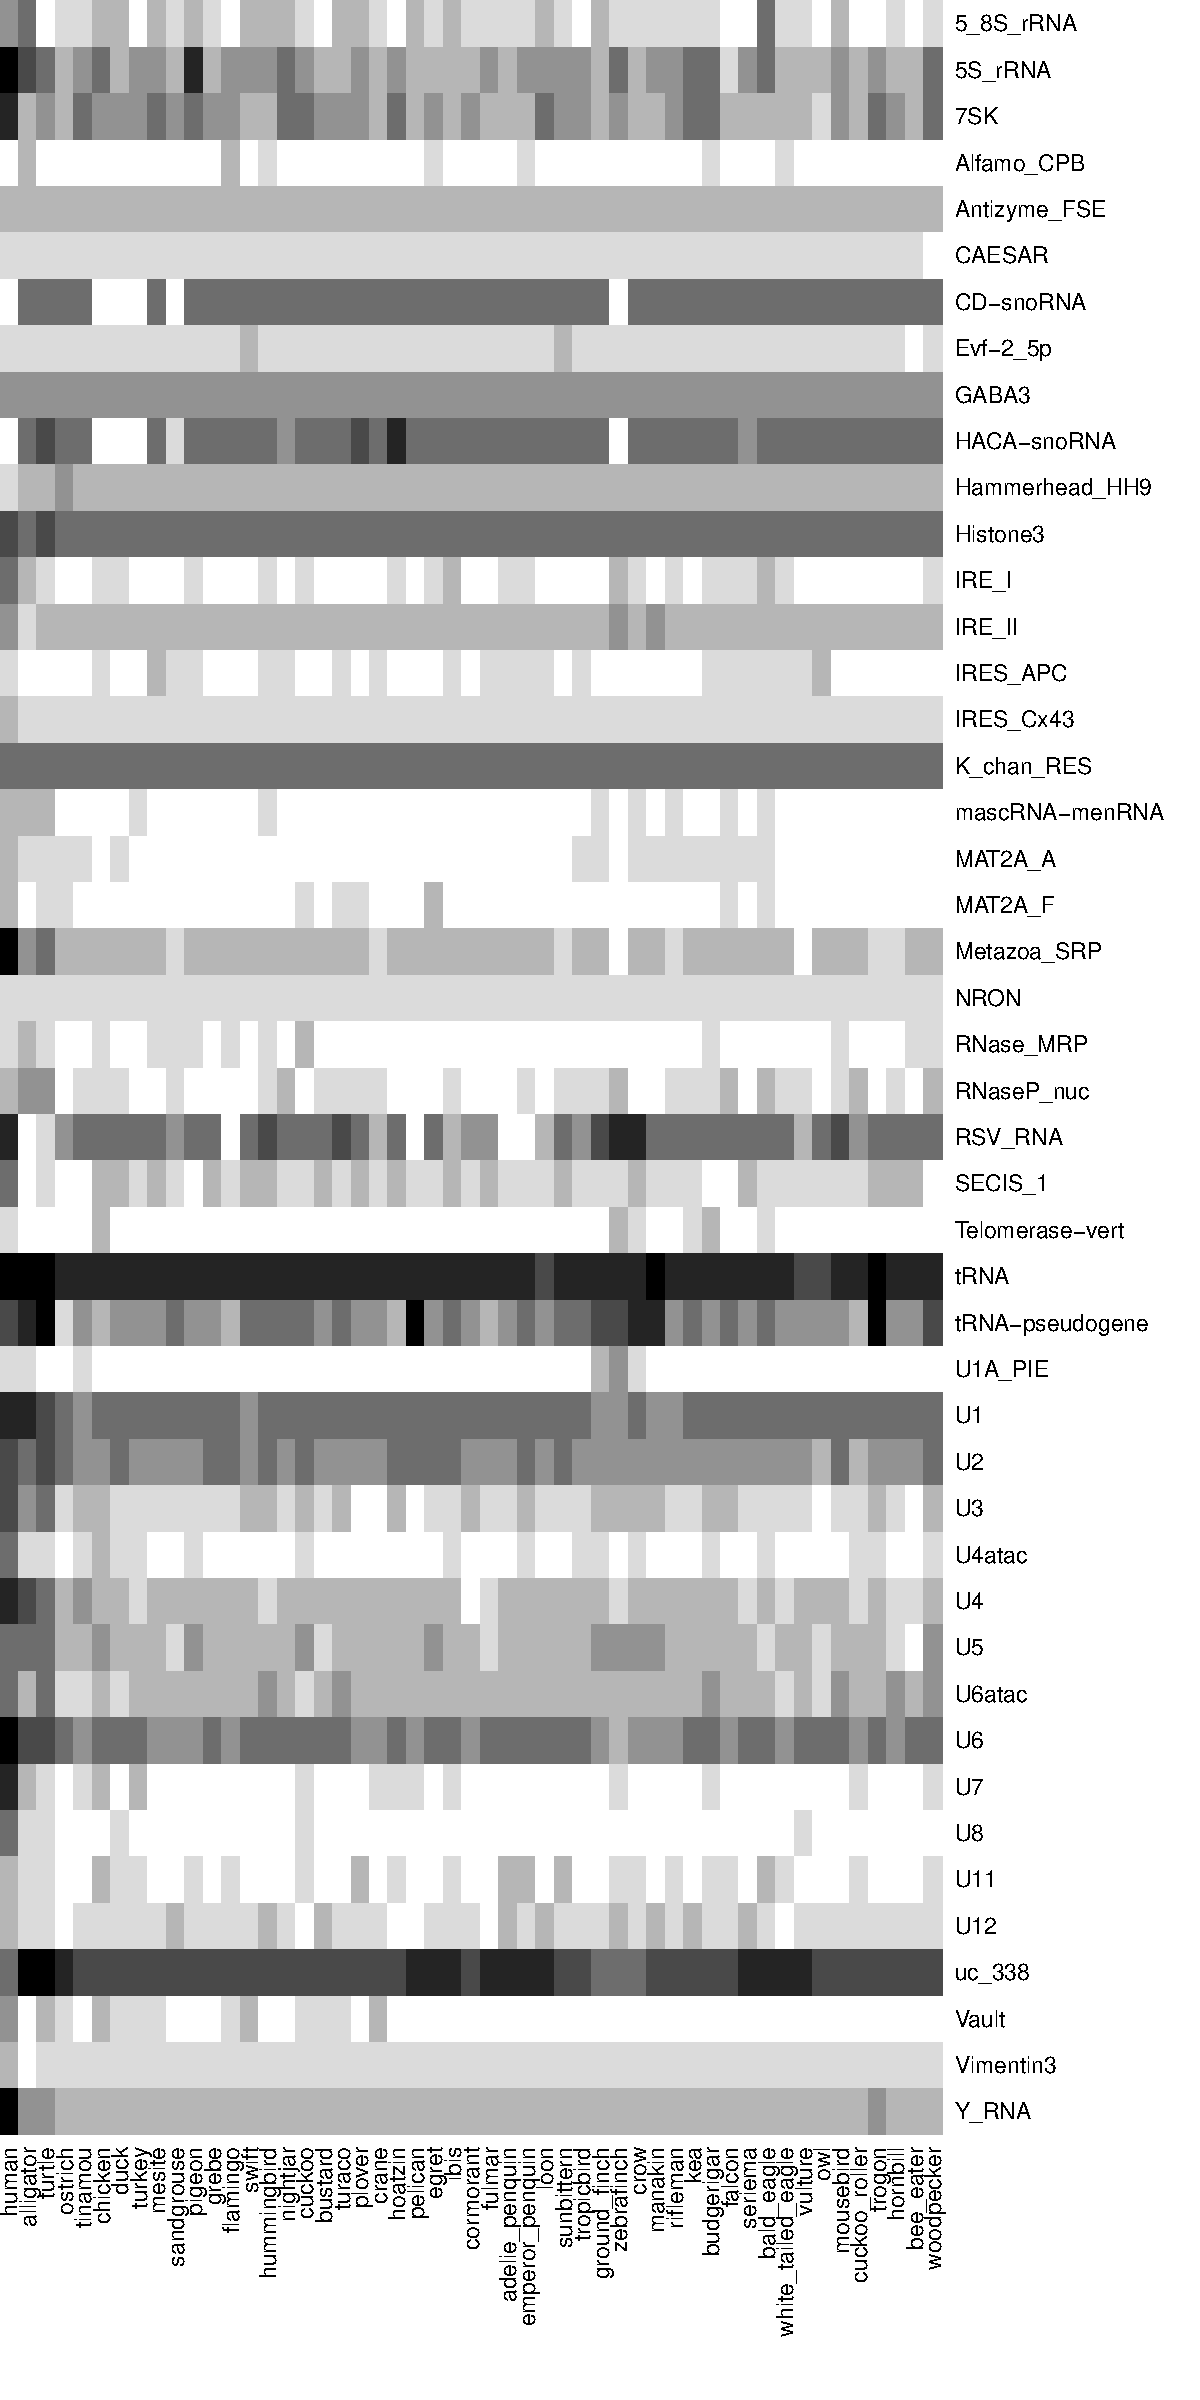
\includegraphics[width=0.4\textwidth]{figures/RNA.pdf}  
  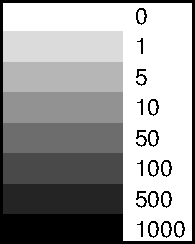
\includegraphics[width=0.1\textwidth]{figures/key2.pdf}
  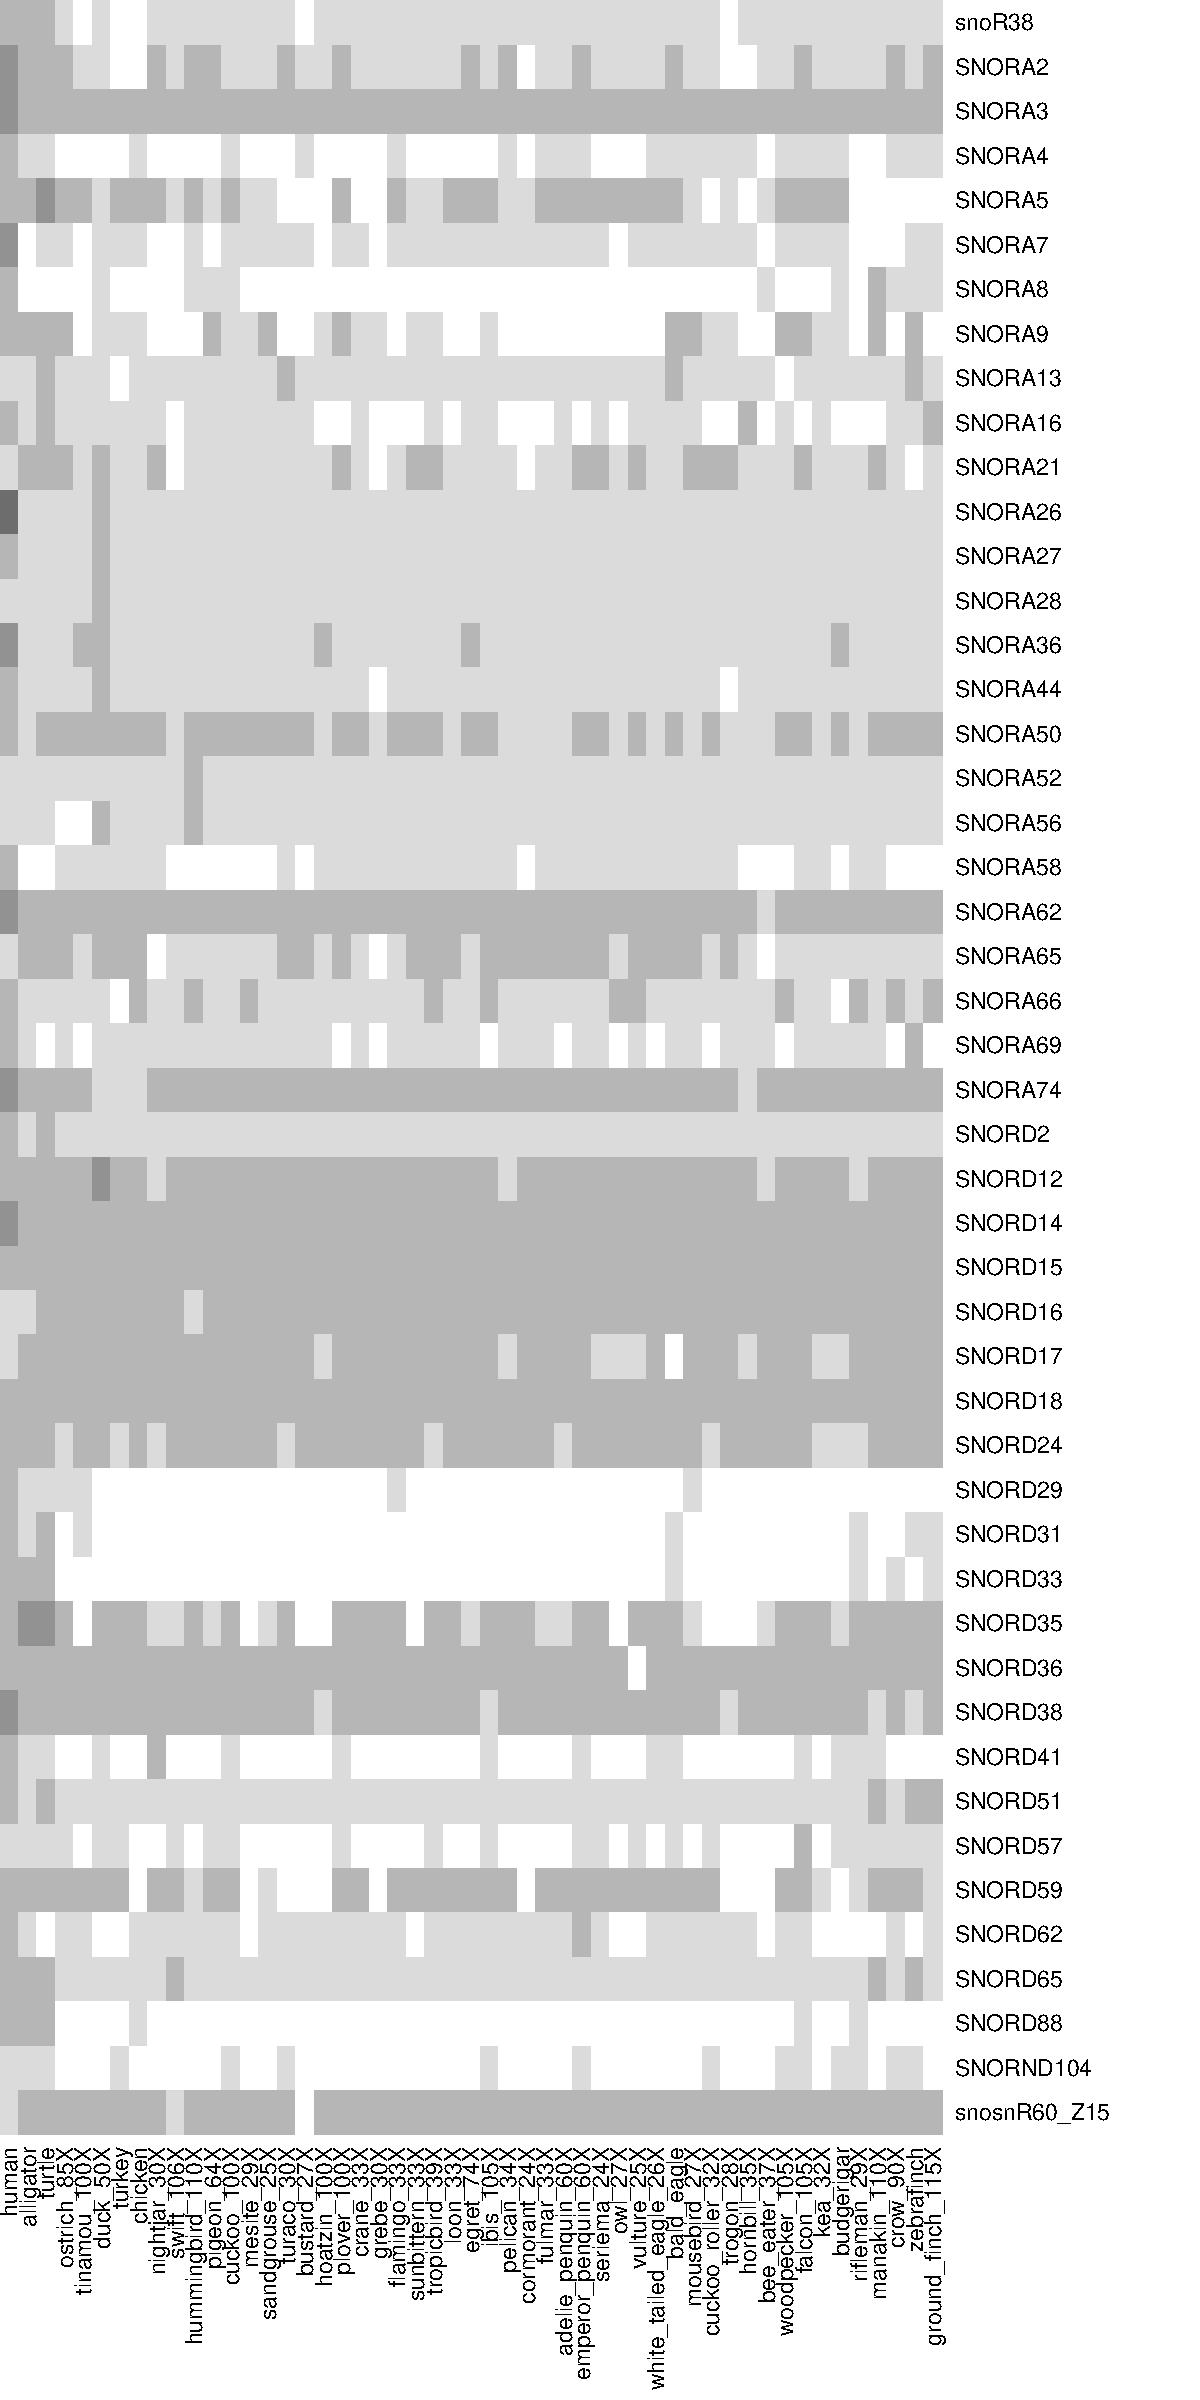
\includegraphics[width=0.4\textwidth]{figures/snoRNA-human-yeast-correspondences.pdf}
  \caption[]{This figure illustrates the number of copies of Rfam and
    tRNAscan annotations for each RNA family in each avian species and
    outgroups. The families are ordered alphabetically vertically and
    the species are in phylogenetic order horizontally. Darker shades
    indicate high copy numbers, lighter shades indicate fewer, white
    indicates no predictions were made.}\label{fig:1}
\end{figure}


%% \begin{figure}[ht]
%%   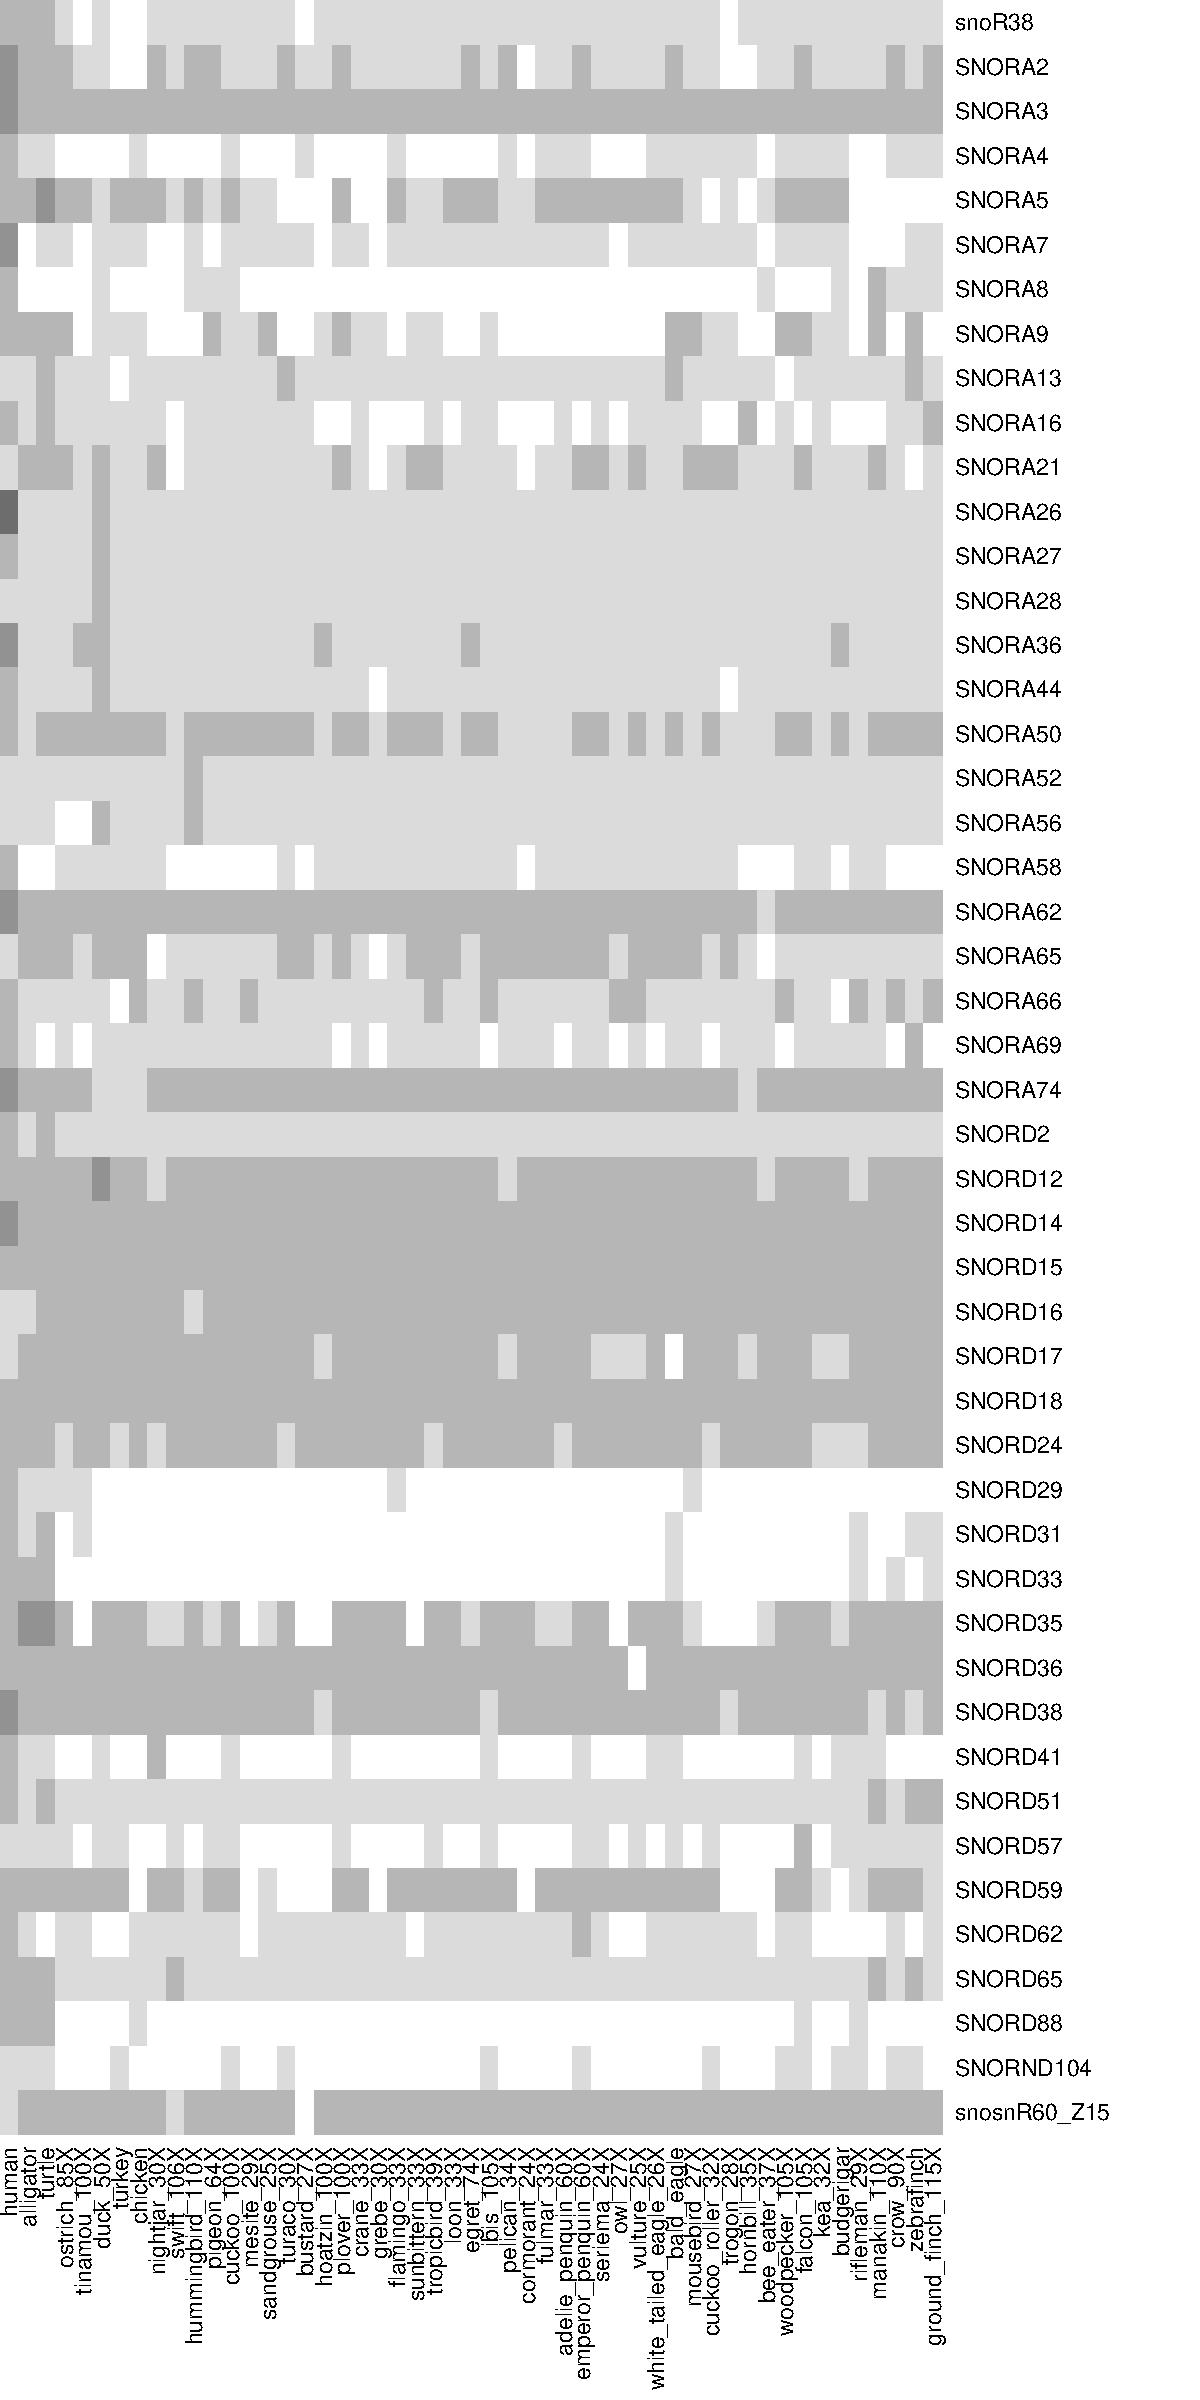
\includegraphics[width=0.65\textwidth]{figures/snoRNA-human-yeast-correspondences.pdf}
%%   \caption[]{.}\label{fig:2}
%% \end{figure}


\begin{figure}[ht]
  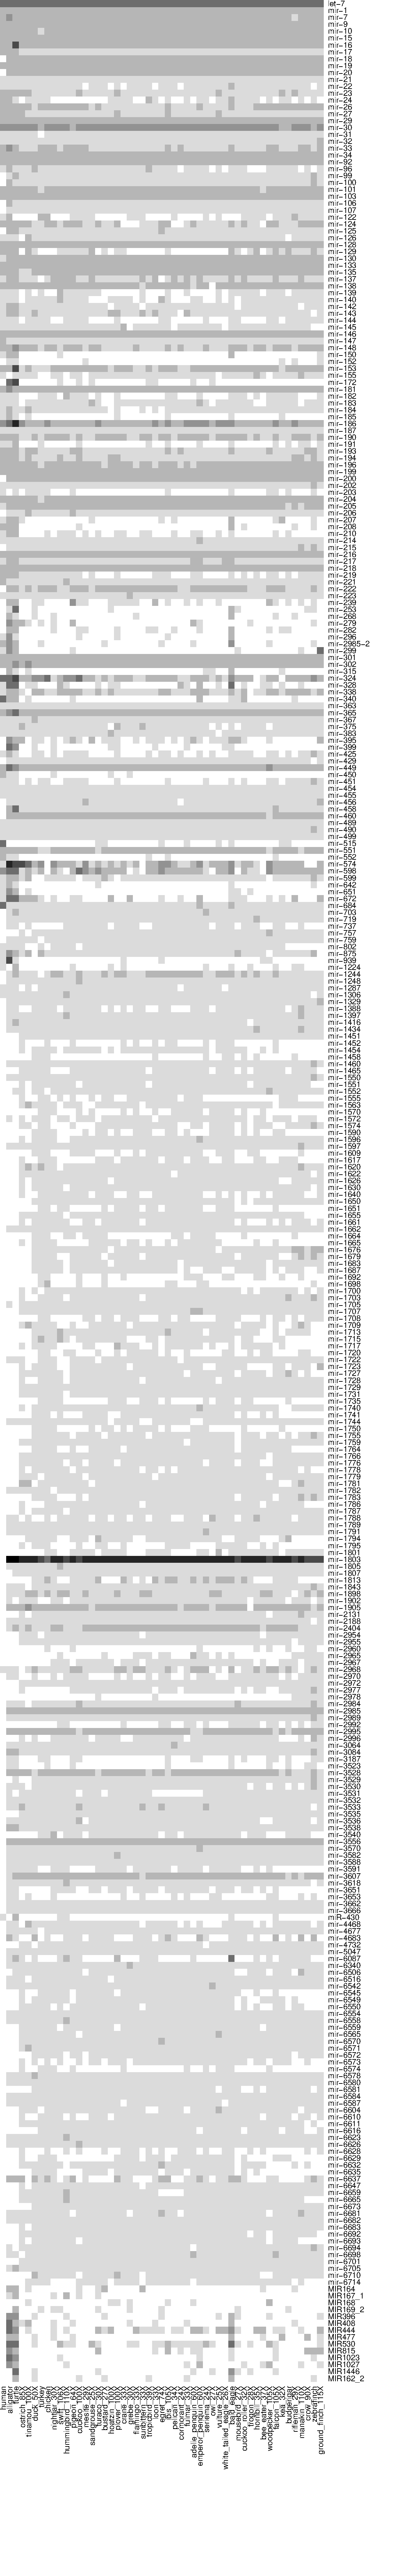
\includegraphics[height=0.95\textheight]{figures/miRNA.pdf}
  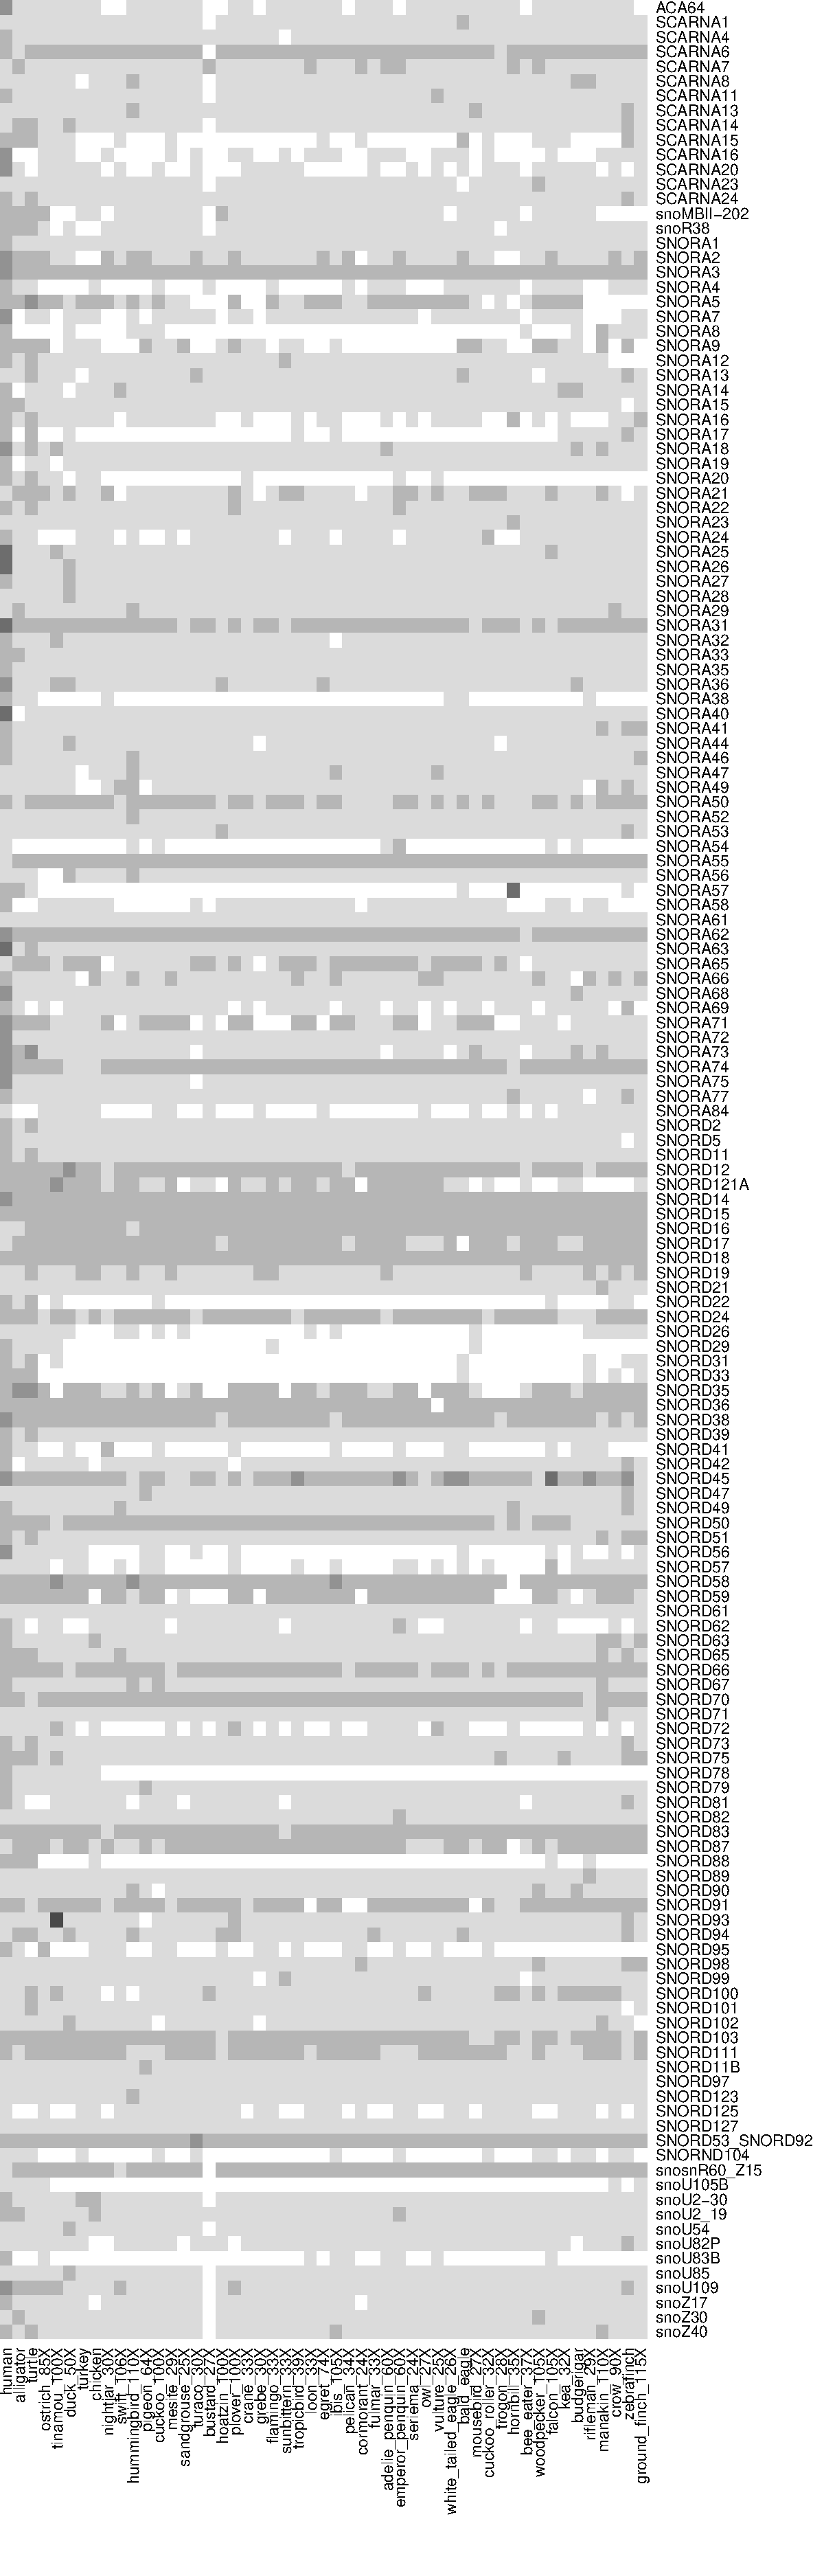
\includegraphics[height=0.95\textheight]{figures/snoRNA.pdf}
  \caption[]{.}\label{fig:3}
\end{figure}

\begin{figure}[ht]
  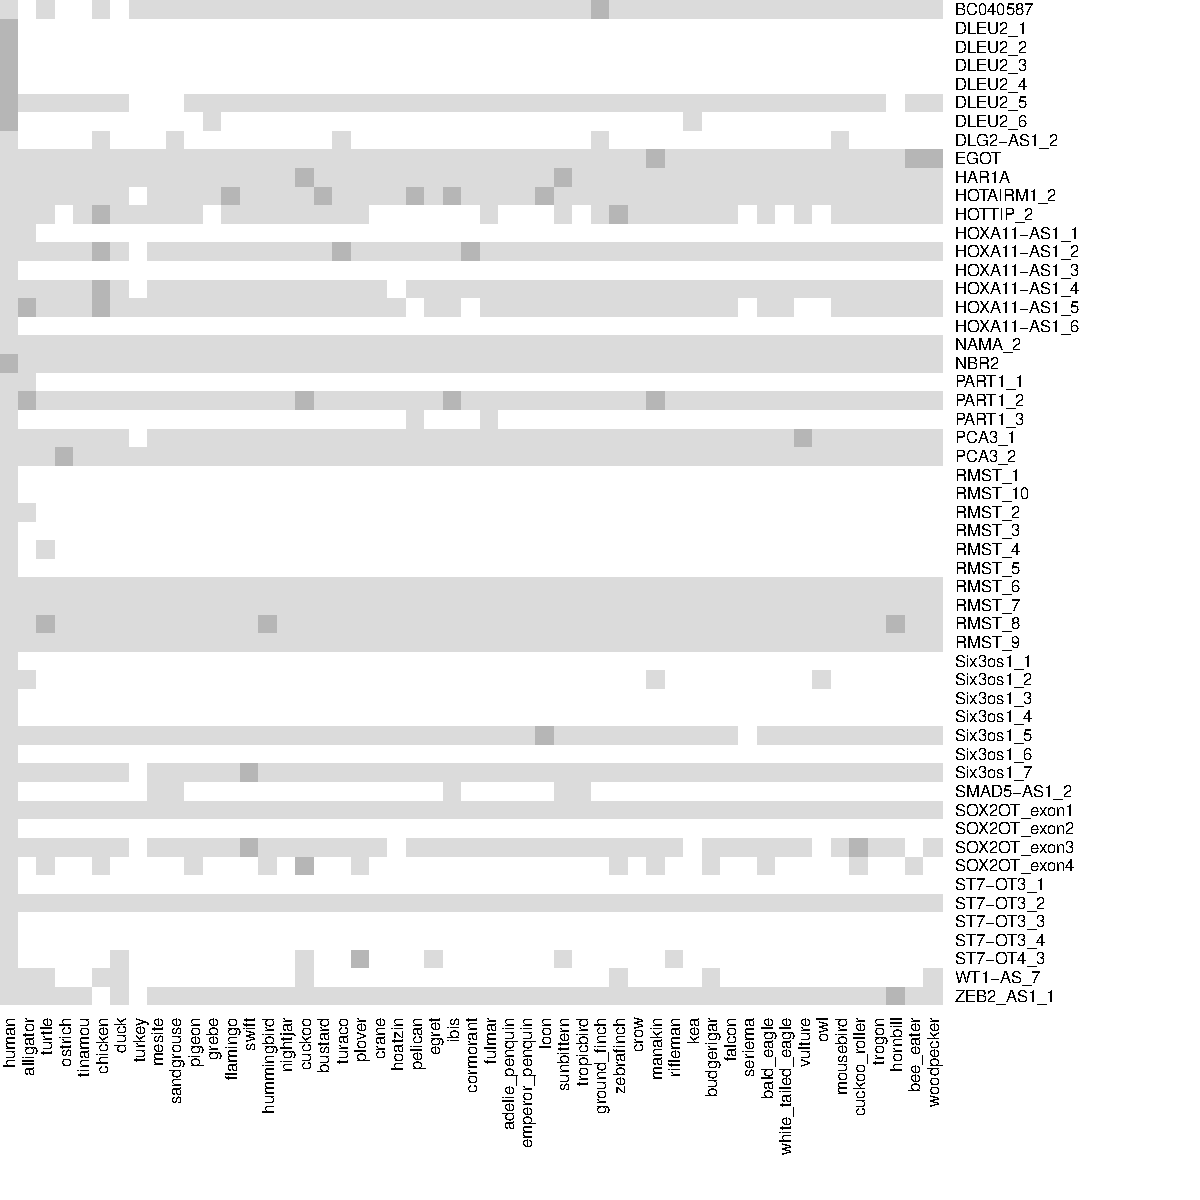
\includegraphics[width=0.45\textwidth]{figures/lncRNA.pdf}
  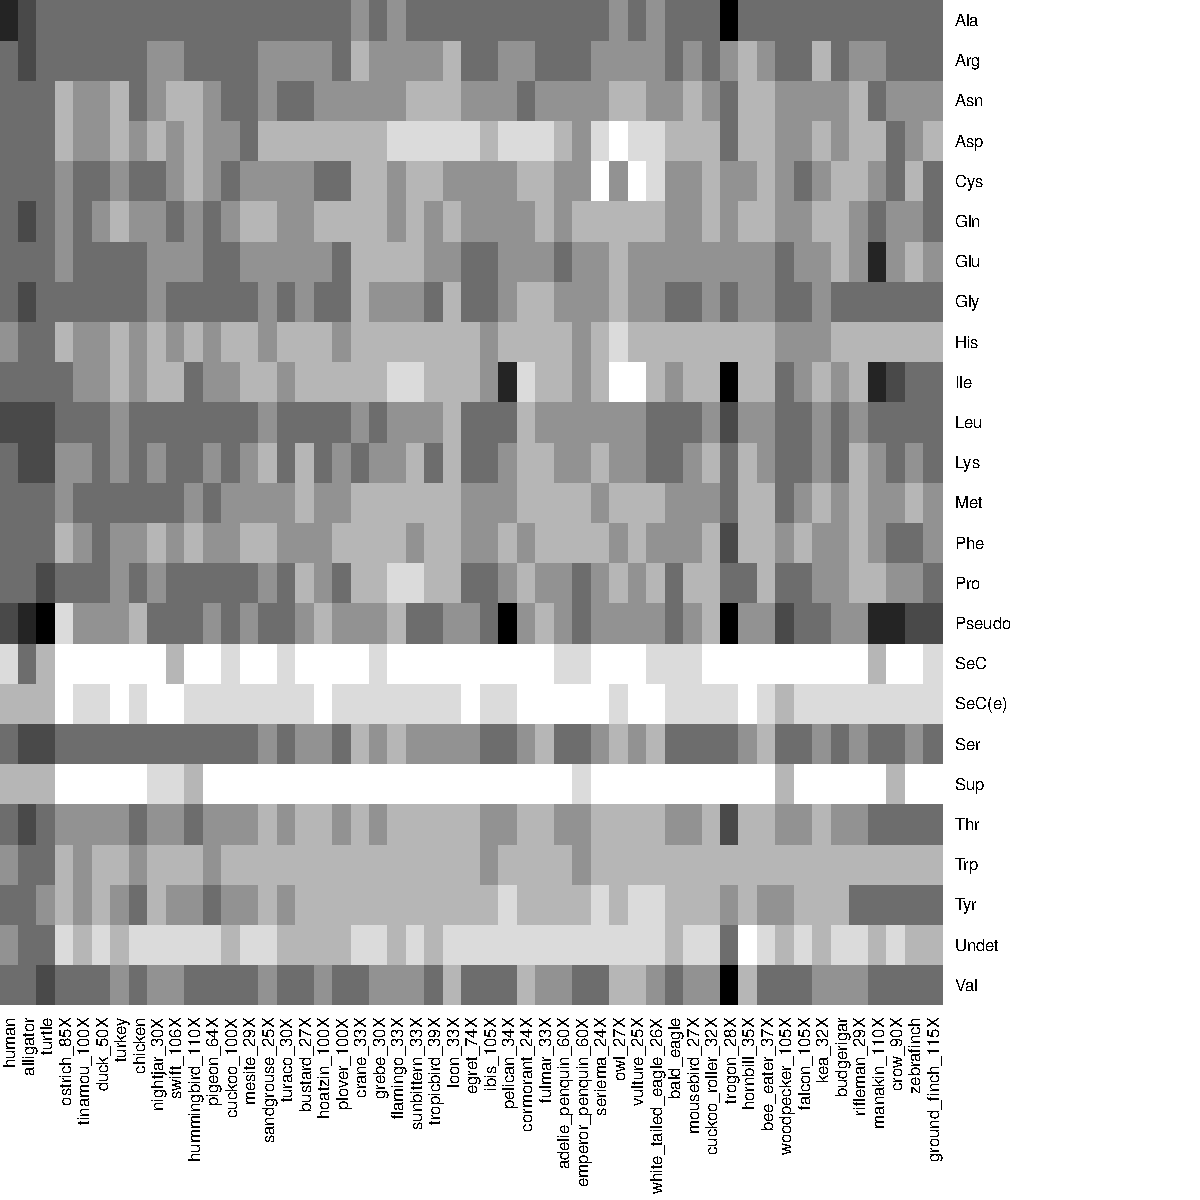
\includegraphics[width=0.45\textwidth]{figures/tRNA.pdf}
  \caption[]{.}\label{fig:5}
\end{figure}



\end{bmcformat}
\end{document}

%%% Local Variables: 
%%% mode: latex
%%% TeX-master: t
%%% End: 

